\documentclass[11pt,]{article}
\usepackage[left=1in,top=1in,right=1in,bottom=1in]{geometry}
\newcommand*{\authorfont}{\fontfamily{phv}\selectfont}
\usepackage[]{mathpazo}


  \usepackage[T1]{fontenc}
  \usepackage[utf8]{inputenc}



\usepackage{abstract}
\renewcommand{\abstractname}{}    % clear the title
\renewcommand{\absnamepos}{empty} % originally center

\renewenvironment{abstract}
 {{%
    \setlength{\leftmargin}{0mm}
    \setlength{\rightmargin}{\leftmargin}%
  }%
  \relax}
 {\endlist}

\makeatletter
\def\@maketitle{%
  \newpage
%  \null
%  \vskip 2em%
%  \begin{center}%
  \let \footnote \thanks
    {\fontsize{18}{20}\selectfont\raggedright  \setlength{\parindent}{0pt} \@title \par}%
}
%\fi
\makeatother




\setcounter{secnumdepth}{0}


\usepackage{graphicx,grffile}
\makeatletter
\def\maxwidth{\ifdim\Gin@nat@width>\linewidth\linewidth\else\Gin@nat@width\fi}
\def\maxheight{\ifdim\Gin@nat@height>\textheight\textheight\else\Gin@nat@height\fi}
\makeatother
% Scale images if necessary, so that they will not overflow the page
% margins by default, and it is still possible to overwrite the defaults
% using explicit options in \includegraphics[width, height, ...]{}
\setkeys{Gin}{width=\maxwidth,height=\maxheight,keepaspectratio}

\title{Political Economy of Mass Transport in a South Asian Megacity: The case
of Dhaka  }



\author{\Large Rushad Faridi\vspace{0.05in} \newline\normalsize\emph{University of Dhaka}  }


\date{}

\usepackage{titlesec}

\titleformat*{\section}{\normalsize\bfseries}
\titleformat*{\subsection}{\normalsize\itshape}
\titleformat*{\subsubsection}{\normalsize\itshape}
\titleformat*{\paragraph}{\normalsize\itshape}
\titleformat*{\subparagraph}{\normalsize\itshape}



\usepackage[style=authoryear]{biblatex}

\addbibresource{/home/rushad/Dropbox/Docs/Research/References/masterRefs.bib}


\newtheorem{hypothesis}{Hypothesis}
\usepackage{setspace}

\makeatletter
\@ifpackageloaded{hyperref}{}{%
\ifxetex
  \PassOptionsToPackage{hyphens}{url}\usepackage[setpagesize=false, % page size defined by xetex
              unicode=false, % unicode breaks when used with xetex
              xetex]{hyperref}
\else
  \PassOptionsToPackage{hyphens}{url}\usepackage[unicode=true]{hyperref}
\fi
}

\@ifpackageloaded{color}{
    \PassOptionsToPackage{usenames,dvipsnames}{color}
}{%
    \usepackage[usenames,dvipsnames]{color}
}
\makeatother
\hypersetup{breaklinks=true,
            bookmarks=true,
            pdfauthor={Rushad Faridi (University of Dhaka)},
             pdfkeywords = {mass transportation, South Asia, Political economy},  
            pdftitle={Political Economy of Mass Transport in a South Asian Megacity: The case
of Dhaka},
            colorlinks=true,
            citecolor=blue,
            urlcolor=blue,
            linkcolor=magenta,
            pdfborder={0 0 0}}
\urlstyle{same}  % don't use monospace font for urls

% set default figure placement to htbp
\makeatletter
\def\fps@figure{htbp}
\makeatother

\usepackage[format=hang,labelformat=empty,labelsep=none]{caption}
%\usepackage{biblatex}
%\addbibresource{../../References/masterRefs.bib}
\usepackage{float}
\let\origfigure\figure
\let\endorigfigure\endfigure
\renewenvironment{figure}[1][2] {
    \expandafter\origfigure\expandafter[H]
} {
    \endorigfigure
}
%\usepackage{draftwatermark}
%\SetWatermarkLightness{.9}
\def\tightlist{}


% add tightlist ----------
\providecommand{\tightlist}{%
\setlength{\itemsep}{0pt}\setlength{\parskip}{0pt}}

\begin{document}
	
% \pagenumbering{arabic}% resets `page` counter to 1 
%
% \maketitle

{% \usefont{T1}{pnc}{m}{n}
\setlength{\parindent}{0pt}
\thispagestyle{plain}
{\fontsize{18}{20}\selectfont\raggedright 
\maketitle  % title \par  

}

{
   \vskip 13.5pt\relax \normalsize\fontsize{11}{12} 
\textbf{\authorfont Rushad Faridi} \hskip 15pt \emph{\small University of Dhaka}   

}

}








\begin{abstract}

    \hbox{\vrule height .2pt width 39.14pc}

    \vskip 8.5pt % \small 

\noindent This article will analyze the dynamics and structure of mass
transportation in a South Asian mega city.It is usually expected that
competition will bring about better service and quality in a market. In
transportation sector in Bangladesh it seemed that competion brought
about the worst possible outcome for transportation. This paper
investigates the reasons behind this phenomenon. We found that this is
actually a classic case of market failure since mass transportation is
essentially a public good with externality effect. Therefore, market
equilibrium resulted into socially inefficient outcome.


\vskip 8.5pt \noindent \emph{Keywords}: mass transportation, South Asia, Political economy \par

    \hbox{\vrule height .2pt width 39.14pc}



\end{abstract}


\vskip 6.5pt


\noindent  \section{Introduction}\label{introduction}

In the month of July, an unique movement started in the streets of
Dhaka, Bangladesh. School and high school kids came to streets
protesting death of two of their friends. These two kids died in the
race of two buses to collect passengers and thus increase the day
revenue. This kids actually ruled the city for a few days.

It is usually expected that competition will bring about better service
and quality in a market. In transportation sector in Bangladesh it
seemed that competion brought about the worst possible outcome for
transportation. This paper investigates the reasons behind this
phenomenon. We found that this is actually a classic case of market
failure since mass transportation is essentially a public good with
externality effect. Therefore, market equilibrium resulted into socially
inefficient outcome.

\section{Key research questions}\label{key-research-questions}

why mass transportation is public good

history and nature of public transporation in Dhaka, Bangldesh

consequences of competition in public transporation

Forms of Public Intervention

International best practices on public transportation management

Employment structure

\section{Current state}\label{current-state}

\subsection{Trips}\label{trips}

A project titled ``Dhaka Urban Transport Network Development'' completed
two surveys in 2009 and 2014 with the support of Japan International
Cooperation Agency (JICA). In Dhaka, every day 33 million trips are
made. Of this 72 percent are made in Buses. Another 15.4 percent are
made in autorickshaw. Therefore, close to 90 percent of the trips are
covered by bus and autorickshaw.

\subsection{Fitness}\label{fitness}

According to Bangladesh Road Transportation
Authority(BRTA)\autocite{anwar_palo_respite_2018}, there are two hundred
and 16 thousand cars which are without fitness. There are two aspects of
fitness. One is external and another is internal or technical. To
provide fitness, BRTA is required to consider 60 different types of
issues. Acording to experts, let alone technical side, if we just
consider external factors, 80-90 percent of Bus and Minibus is unfit to
move around.

From \autocite{anwar_palo_words_2018} After assuming office in 2009, the
Bangladesh Awami League (AL)-led government announced that buses older
than 20 years would be shortly withdrawn. In 2011, Obaidul Quader, also
the president of road transport advisory council, took office of the
road transport and bridges ministry.

Quader, after one year of taking office, came up with an announcement to
withdraw all unfit vehicles. He made the same announcement in a meeting
of the road transport advisory council in June of the following year,
also the last year of this government's previous tenure.

Sometime close to the end of the tenure, minister Quader said, ``We
cannot do everything now even if we want to.''

The AL came to power again after the 5 January elections in 2014 and
Quader was handed over the responsibilities of the same ministry. Then,
once again he made the announcement in a programme to withdraw unfit
vehicles to ease traffic congestion in the Dhaka airport area. An
11-member taskforce, headed by the then chairman of the Bangladesh Road
Transport Authority (BRTA), was also formed.

\subsection{No. of buses}\label{no.-of-buses}

Over the years number of buses are decereasing. At 2015, bus numbers
were reduced to 4500. This situation is quite strange. The factors
behind this lower buses is lower profits, uncertainty on political
unrest, hooliganism, etc.

Everyday, around 10 thousand buses are entering our city. Over the
years, no. of buses are getting reduced. Bus company manufacturers and
sellers might be an interested part to all this.

\subsection{How other countries solved the
problem}\label{how-other-countries-solved-the-problem}

what was the experience of these following cities?

Dhaka, Kolkata, Bombay, Delhi, Karachi what is their experience?

\subsection{Planning}\label{planning}

Who is planning for whom? How the planning is done? Why it is not done?

\section{Employment structure}\label{employment-structure}

This article will focus on the dynamics of employment structure in a
South Asian mega city. In July, 2018 a bus killed two school children in
a race to collect more passengers. It brought down protests throughout
the country and particularly in Dhaka, the school students took over the
control of the streets replacing the traffic surgeons. It created a
great political upheaval in Bangladesh. The objective of this paper is
to look into the economic incentive of Bus operators that lead to this
stiff aggressively competitive behaviors which led to the tragic
incident. We will look into the current employment structure which is
actually determined by the whole mass transportation industry.

\subsection{Current state}\label{current-state-1}

Describe the administrative structure of

According to \textcite{anwar_palo_words_2018}, BRTA data shows there are
3.30 million vehicles in the country. In the same vein, according to
BRTC, there are 35,000 buses and mini buses, half of which operate
outside Dhaka.According to Bangladesh Road Transport Authority (BRTA), a
total of 7,937 bus and mini buses ply along 246 routes in Dhaka and its
adjacent areas.

Bus, CNG-run auto-rickshaw and rickshaw are three mainstays of public
transport in the capital. Bus and auto-rickshaw contribute to as many as
87.40 per cent of road transport communication in Dhaka while bus alone
makes 72 per cent.\footnote{These information comes from two major
  studies done by Dhaka Transport Coordination Board (DTCB) at the
  behest of Japan International Cooperation Agency (JICA). The first was
  completed in 2010 \autocite{dtcb_preparatory_2010} follwed up by
  \autocite{dtcb_preparatory_2011}. Considering this situation the
  government of Bangladesh formulated a `Strategic Transportation Plan'
  (STP) in cooperation with the World Bank in 2005. The implementing
  agency is Dhaka Transport Coordination Board (DTCB) under the Ministry
  of Communications (MOC). The STP prepared `Urban Transportation
  Policy' for 20 years (2004--2024), and identified priority issues such
  as improvement of mass transit system (buses and rail transportations)
  , development of urban expressway and establishment of organization in
  implementation and maintenance/operation of the projects. Since the
  STP has already received the official approval of the government of
  Bangladesh, it is}

Many bus owners have one or two buses. Dhaka Metropolitan Regional
Transport Committee gives permission for movement of the vehicles. The
committee members include police and representatives from BRTA,
different departments of the government and bus owners and workers.

After the application for permission, traffic police, the opinions of
bus owners-workers and the clout of the applicants are taken into
consideration.

The route permission was given after setting certain conditions of the
Motor Vehicle Act, without any consideration of passengers' route
demands, population density or road capacity.

Due to unplanned and unnecessary routes and innumerable owners, the
buses enter unhealthy competition. As there are many owners under the
same company, the drivers of buses join in a competition as to who will
pick up passengers first and this causes road accidents.

About 255 bus operators ply in the streets of Dhaka with around 8000
buses. There are around 129 routes on which this buses runs through.
There are no planned structure on which bus operator will maintain which
route, there are no time schedule. Unbriddled competition has led to
total chaos in this sector. This immensely affected the behaviour of
drivers who are at the heart of maintaining safety on the road. The
channel through which this drivers are affected is mainly their main
source of livelihood, the salary earned from driving these buses. It is
how their earning is determined will affect current state. Therefore the
main focus of our discussion is the remuneration packages that is
offered to these drivers.

\subsection{Existing employment
structures}\label{existing-employment-structures}

Almost all of the bus operators in developing countries main revenue
collection comes from fare. Therefore, a bus operation is considered
successful only if it generates enough revenue from fare. But it is not
always possible to monitor the bus crew. There is a strong possiblity
that they won't report all the revenue from bus. There may be also false
issuance of tickets thereby defrauding the operators.

To counter the leakage of salary, the bus owners/operators offer drivers
a share of fare revenue. it becomes salary or part of the salary. it
creates incentive for the drivers for to report all the revenue but it
falls short of solving the revenue leakage. monetary benefit of the
driver is directly related to number of passengers a bus can have. in
the absence of proper law enforcement and service monitoring, this will
lead to aggressive driving, over-speeding and leads to uncomfortable,
unreliable and unsafe travel.

salary system of conductor and driver is similar. therefore they are all
considered as whole.

According to \textcite{htun_influence_2012}, there are mainly four types
of driver salary system exists in the developing countries

\begin{itemize}
\item
  Share of fare revenue
\item
  Bus fleet rental system
\item
  Fixed salary system
\item
  Fixed salary and incentives
\end{itemize}

In the following, we find a table where main features are highlighted:

\begin{figure}
\centering
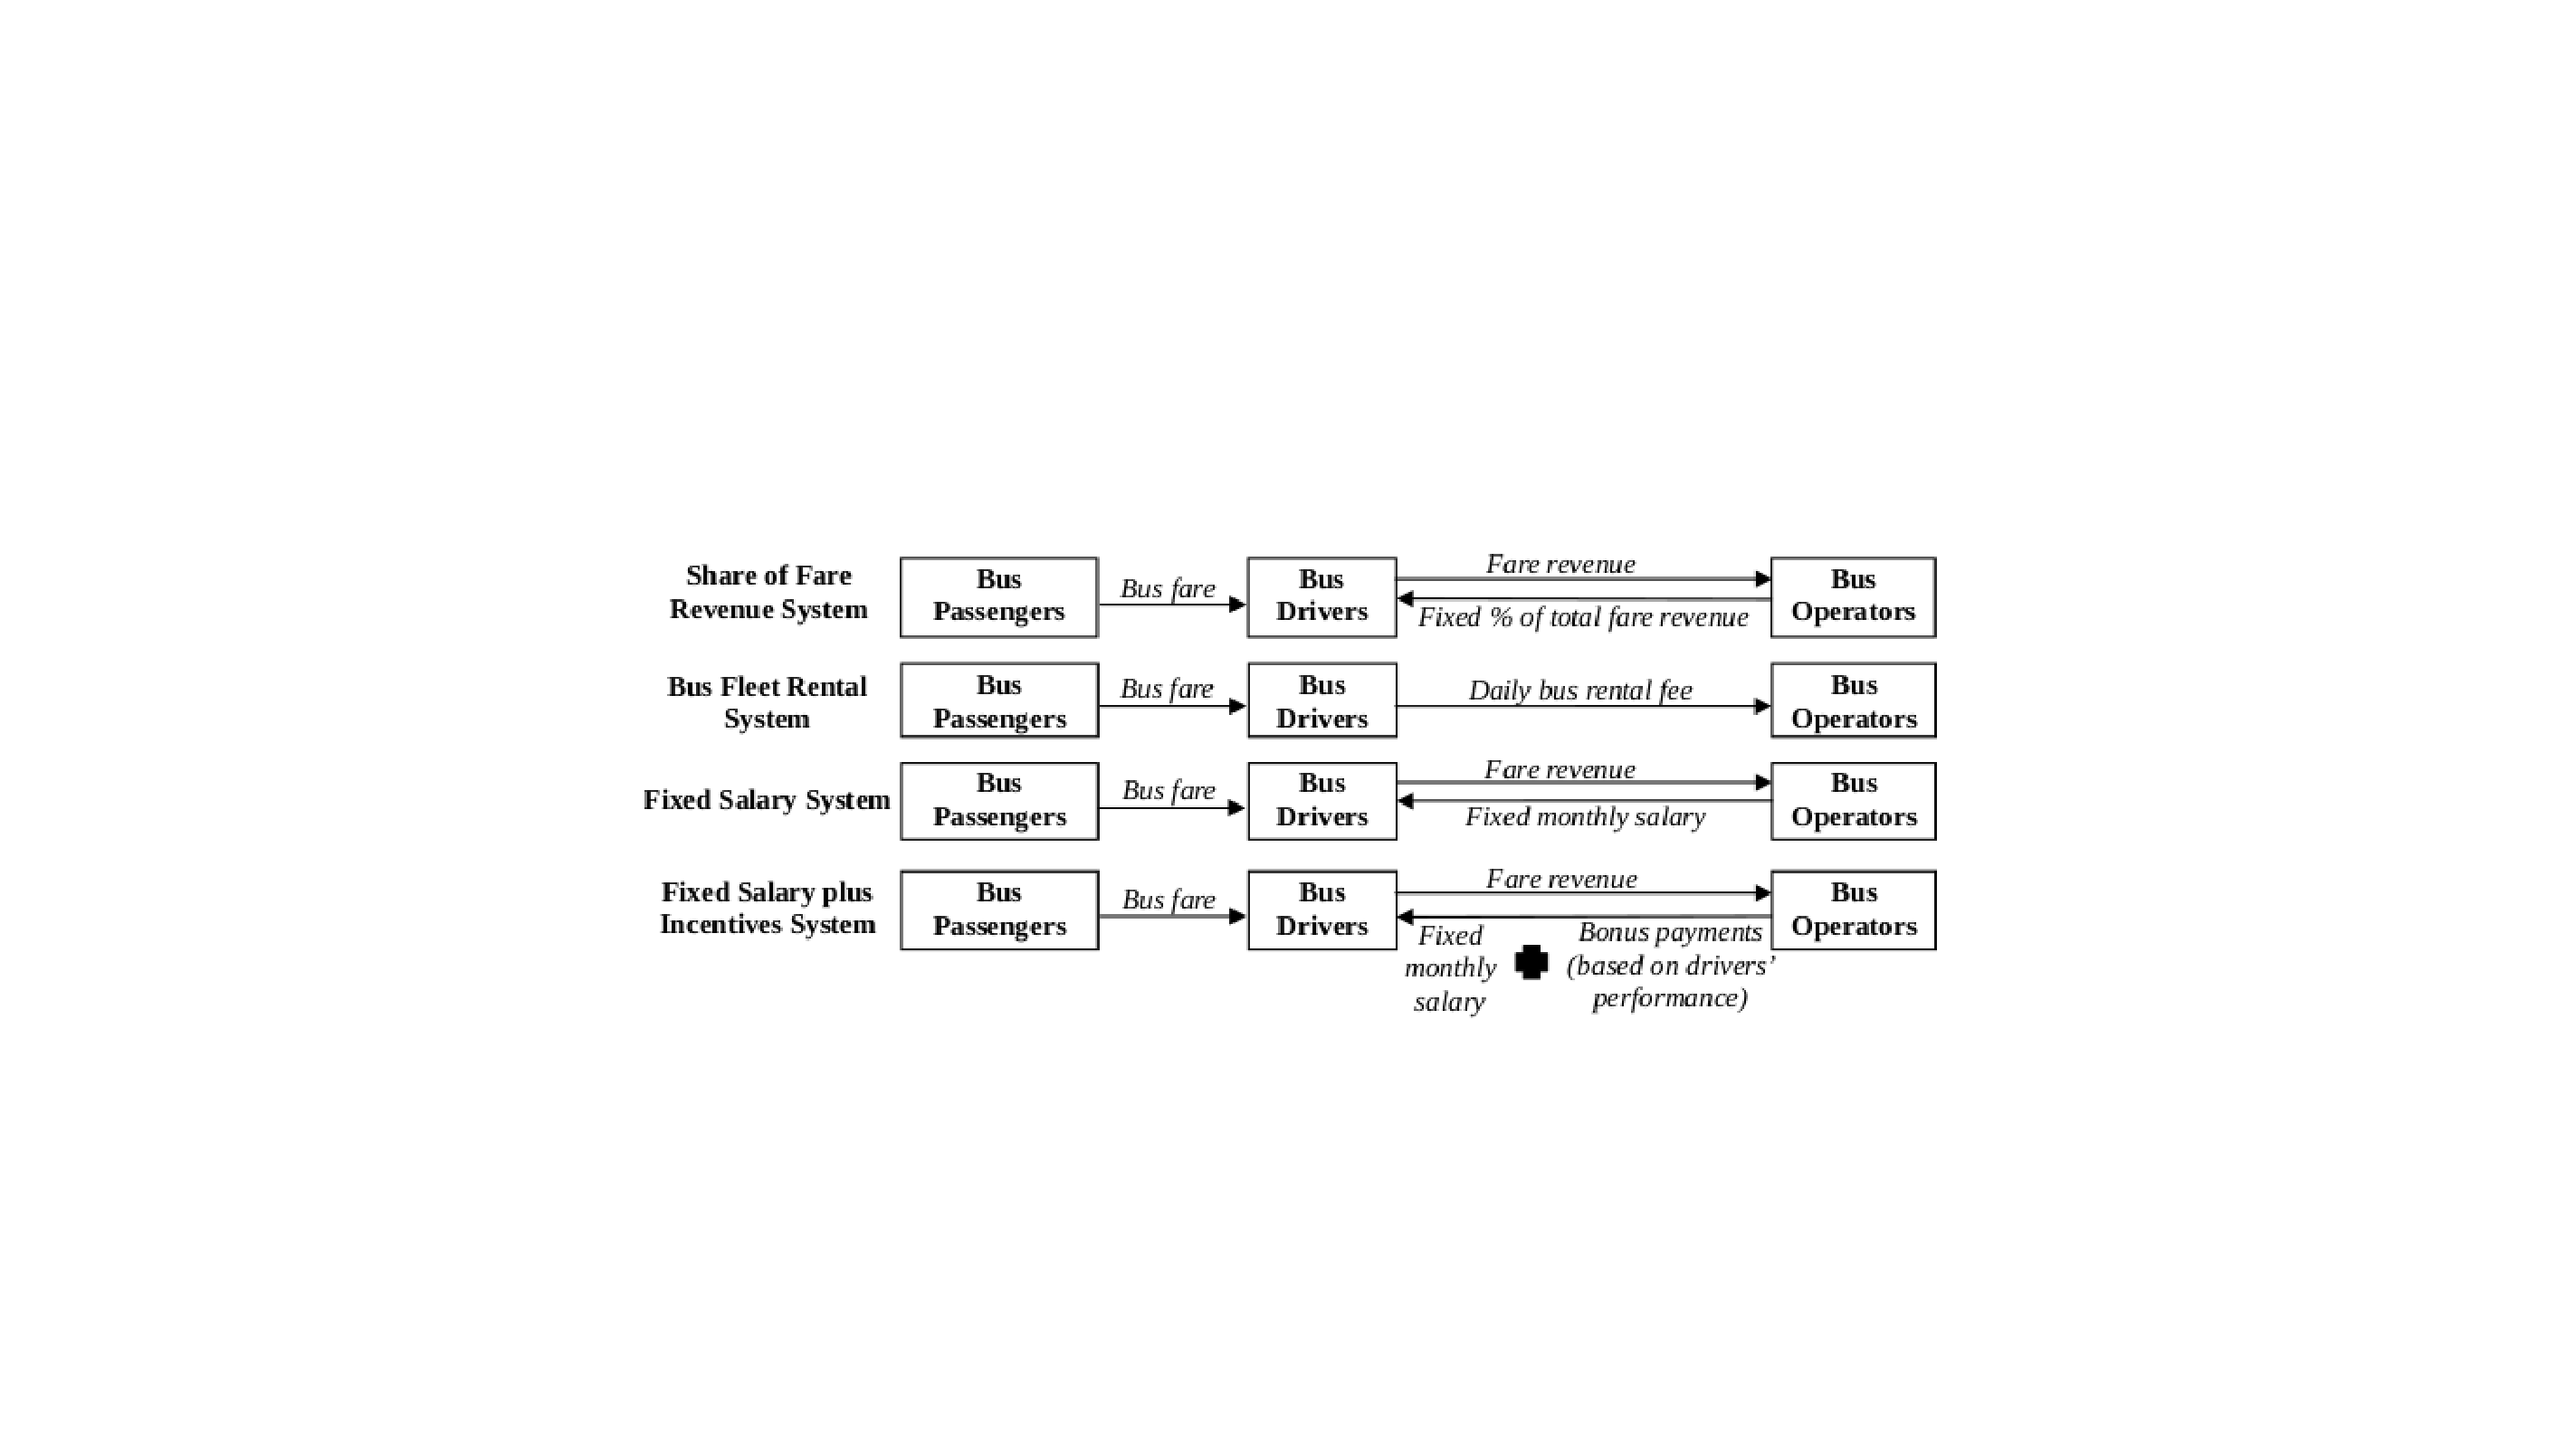
\includegraphics{./figures/emp_str_flow.pdf}
\caption{\textbf{Figure 1:} fig\_title}
\end{figure}

\subsubsection{Share of fare revenue}\label{share-of-fare-revenue}

Major advantage of this system is that the driver has strong incentive
to provide effort since they share of the pie will increase as the pie
itself gets larger. At the same time it causes some undesirable and in
some cases dangerous driving practices by the drivers. Number of bus
passengers determine the salary of bus driver and bus drivers try to
maximize this by collecting as much as passengers as possible. In that
regard, following driving practices are observed: - Drivers race to next
bus stop to beal rival's vehicles in picking up passengers - They stop
for long periods of time at bus stops to wait for more passengers until
a competitor appears - They often stop at unauthorised places along the
raod if there is a passenger.

The consequence of this driver behavior can create enormous safety
problem. There is fairly undisputable evidence of high accident rates
associated with this nature of competiton. Such reckless driving makes
the passengers even more uncomfortable and unsafe and disturbs traffic
flow. This reduces road capacity and thereby causing traffic congestion
in urban areas and can have a serious deterimental effect on bus
services. Moreover using vehicles intensively can increase vehicle
maintenance costs and results in more frequent breakdowns of vehicles
during bus operations. its true drivers are highly motivated but the
thing is that it does not ensure high revenue. the crews still have
incentive to report lower revenue.

As mentioned above, the principal advantage of this system is that
drivers are more motivated to work harder while also providing bus
operators with the incentive to earn better returns from their bus
operations by encouraging their drivers motivation to work. Furthermore,
this system can give them strong incentive to combat fare evasion by
passengers. However such system is not always effective deterrant
against pilferage of revenue since it depends on the honesty of drivers
to remit all fare revenue collected. In Santiago,this happened.

\subsubsection{Bus fleet rental}\label{bus-fleet-rental}

a bus is operated by a driver who rents it on a daily basis from bus
operators for a fixed daily sum. the driver can retain any surplus
revenu as their remuneration. this is for the conventional bus in
jakarta. they take a lot of time to collect passengers and then drive
very fast. advantage for the owners, they need not monitor the revenue

\subsubsection{Fixed salary system:}\label{fixed-salary-system}

weakest incentive for driver to provide effort, there is also revenue
leakage problem

\subsubsection{Fixed salary plus incentives
system}\label{fixed-salary-plus-incentives-system}

bonus payments for reduced fuel consumption, fewer breakdowns, fewer
accidents. but the revenue leakage problem still persists.

For empirial evidence of how the above system actually works in real
life, \textcite{johnson_war_2015} compared two systems of bus driver
compensation in Santiago, Chile. The first system is called payment
based on per passenger transported. This is akin to shared passenger
fare system. The second one is fixed wage is the same as fixed salary
system. Examining these systems on similar routes in Santiago
\textcite{johnson_war_2015} observed that shared passenger fare system
leads to 67\% more accidents per kilometer driven compared to fixed
salary system.




\newpage
\singlespacing 
\printbibliography[title=References]

\end{document}
